\subsection{Polynomial Decusping}
\begin{frame}[t]{Description}

\begin{itemize}
    \item Rodded 3$\times$3 assembly case used to plot generate correction factors based on rod position
    \begin{itemize}
        \item One set of calculations performed with refined mesh to eliminate cusping effects
        \item Second set done with coarse mesh
        \item Percent change in \keff{} plotted against percent change in volume fraction for each set of calculations
        \item Difference in curves used to reduce volume fraction during rod homogenization to reduce cusping effects
    \end{itemize}
    \item Sixth order polynomial curves generated for AIC, \bfc{}, and tungsten rods
\end{itemize}

\end{frame}

%%%%%%%%%%%%%%%%%%%%%%%%%%%%%%%%%%%%%%%%%%%%%%%%%%%%%%%%%%%%%%%%%%%%%%%%%%%%%%%%%

\begin{frame}[t]{Polynomials}
    
\begin{center}
    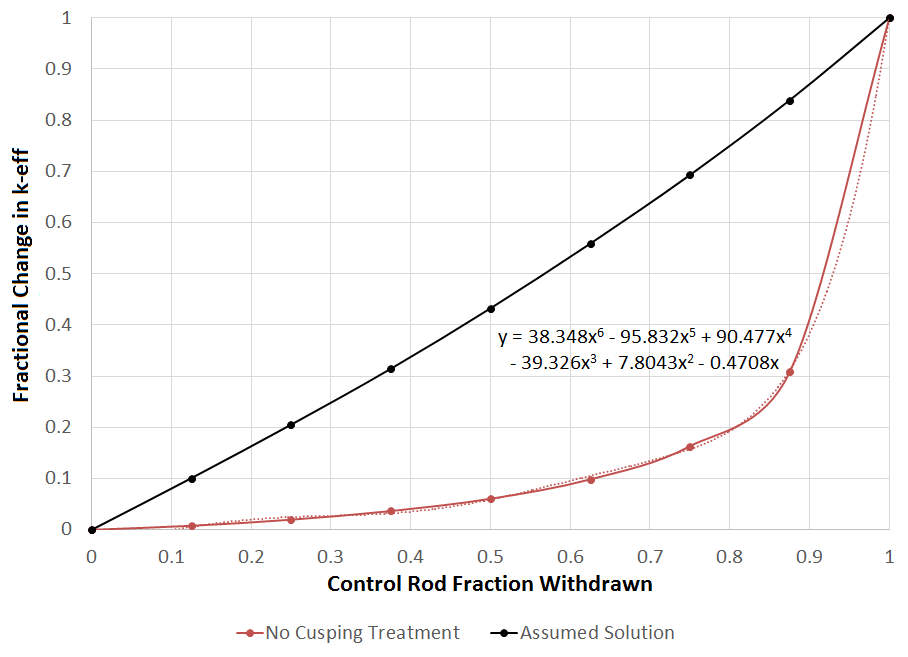
\includegraphics[width=0.8\textwidth]{polynomial_curves.png}
\end{center}
    
\end{frame}

%%%%%%%%%%%%%%%%%%%%%%%%%%%%%%%%%%%%%%%%%%%%%%%%%%%%%%%%%%%%%%%%%%%%%%%%%%%%%%%%%

\subsection{Subplane Collision Probabilities}

\begin{frame}[t]{Subplane Decusping}
    
    \begin{itemize}
        \item Modifications made to subplane scheme \cite{Graham2017Improvementofthe2D/1DMethodUsingtheSub-PlaneScheme,Graham2017RodDecuspingTechniquesforthe2D/1DMethod} to treat axial effects of rod cusping
        \begin{itemize}
            \item Homogenization still uses MOC flux with axial shape factor, but 
            with heterogeneous rodded or unrodded cross sections
            \item Projection rehomogenizes cross sections in partially rodded nodes 
            after CMFD calculation
        \end{itemize}
        \begin{equation}\label{e:nTRACERdecusping}
        \overline{\Sigma_i} = \frac{\phi_{rad,i}^R \phi_{ax,i}^R \Sigma_i^R h^R + \phi_{rad,i}^U \phi_{ax,i}^U \Sigma_i^U h^U}{\phi_{rad,i}^R \phi_{ax,i}^R h^R + \phi_{rad,i}^U \phi_{ax,i}^U h^U} \nonumber
        \end{equation}
    \end{itemize}
    
\end{frame}

%%%%%%%%%%%%%%%%%%%%%%%%%%%%%%%%%%%%%%%%%%%%%%%%%%%%%%%%%%%%%%%%%%%%%%%%%%%%%%%%%

\begin{frame}[t]{Collision Probabilities Decusping}
    
    \begin{columns}
        \begin{column}{0.45\textwidth}
            \begin{itemize}
                \item Sub-plane modifications only capture axial effects
                \begin{itemize}
                    \item MOC uses homogenized cross section
                    \item Radial shape does not accurately reflect either region
                \end{itemize}
                \item 1D collision probabilities (CP) introduced to generate radial 
                shapes
                \begin{itemize}
                    \item Generates radial flux profile for rodded and unrodded region
                    \item Radial profiles used in CMFD homogenization
                    \item Fast calculation
                \end{itemize}
            \end{itemize}
        \end{column}
        \begin{column}{0.55\textwidth}
            \begin{figure}[h]
                \centering
                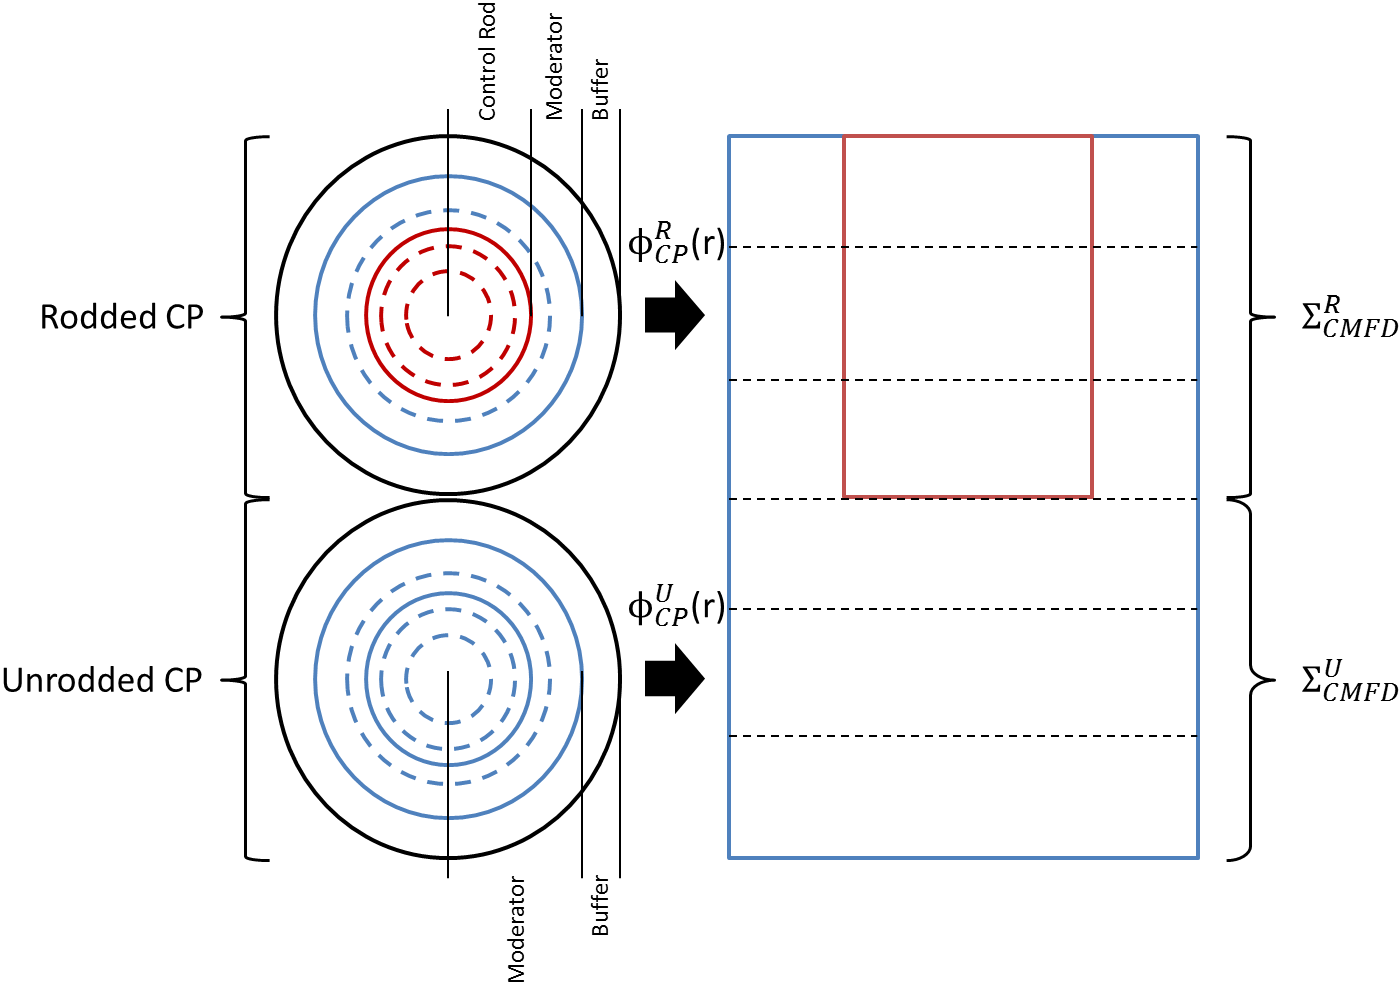
\includegraphics[width=\textwidth]{CPdecusp.png}
            \end{figure}
        \end{column}
    \end{columns}
    
\end{frame}

%%%%%%%%%%%%%%%%%%%%%%%%%%%%%%%%%%%%%%%%%%%%%%%%%%%%%%%%%%%%%%%%%%%%%%%%%%%%%%%%

\subsection{Subray Method of Characteristics}
\begin{frame}[t]{Description}

\begin{itemize}
    \item Other methods do not correctly address the MOC calculation
    \begin{itemize}
        \item Homogenized cross sections are still used for 2D MOC
        \item Flux shape from MOC does not accurately represent rodded or unrodded flux
    \end{itemize}
    \item To improve MOC solutions, heterogeneous cross sections and sources must be accounted for
    \item MOC rays can be split into subrays in the vicinity of partially rodded regions
    \item Because of exponentials in MOC solution, rays can be recombined after rod
\end{itemize}

\end{frame}

%%%%%%%%%%%%%%%%%%%%%%%%%%%%%%%%%%%%%%%%%%%%%%%%%%%%%%%%%%%%%%%%%%%%%%%%%%%%%%%%

\begin{frame}
    
\begin{center}
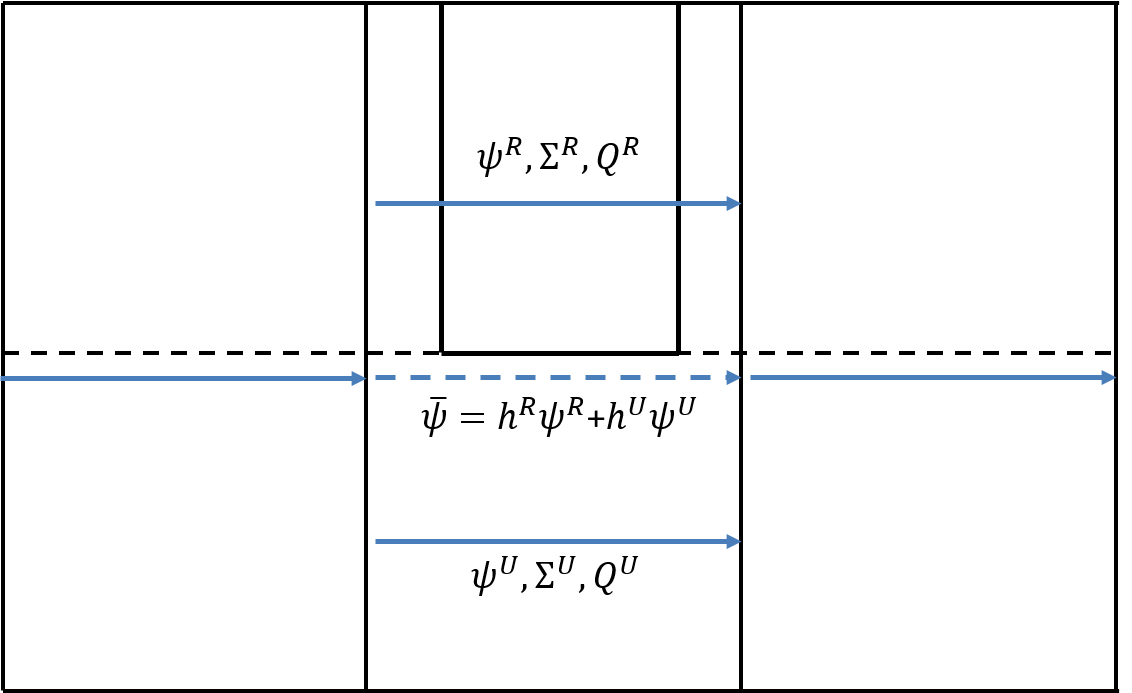
\includegraphics[width=0.8\textwidth]{sub-ray_illustration.png}
\end{center}

\end{frame}

%%%%%%%%%%%%%%%%%%%%%%%%%%%%%%%%%%%%%%%%%%%%%%%%%%%%%%%%%%%%%%%%%%%%%%%%%%%%%%%%

\begin{frame}[t]{2D/1D Modifications}
    
    \begin{itemize}
        \item New MOC sweeper that duplicates long rays using axial volume fractions to average rays together
        \item Fluxes, cross sections, and sources stored for subregions that subrays pass through
        \item CMFD projection used to calculate subregion fluxes and generate subregion sources
        \item Subplane CMFD/P$_3$ results used to calculate axial TL sources in subregions
        \item Option added to control how far away from rod subray continues to be used
    \end{itemize}

\end{frame}

%%%%%%%%%%%%%%%%%%%%%%%%%%%%%%%%%%%%%%%%%%%%%%%%%%%%%%%%%%%%%%%%%%%%%%%%%%%%%%%%

\begin{frame}[t]{Recombination}

\begin{center}
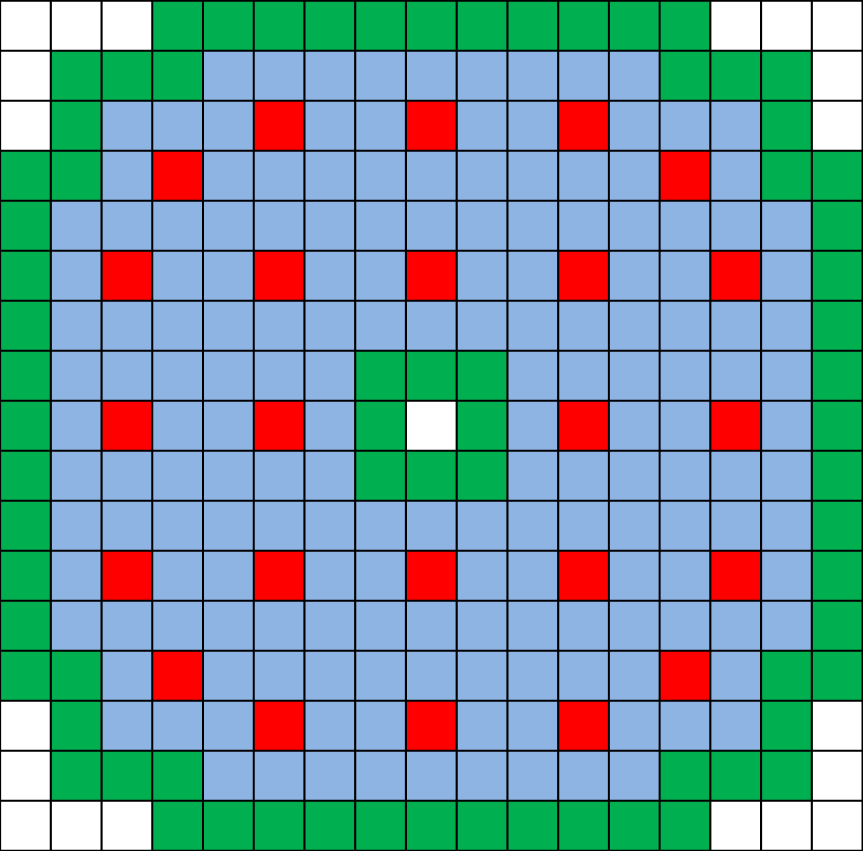
\includegraphics[width=0.5\textwidth]{recombination.png}
\end{center}

\end{frame}